% !TEX TS-program = pdflatex
% !TEX encoding = UTF-8 Unicode

% This is a simple template for a LaTeX document using the "article" class.
% See "book", "report", "letter" for other types of document.

\documentclass[11pt]{article} % use larger type; default would be 10pt

\usepackage[utf8]{inputenc} % set input encoding (not needed with XeLaTeX)
\usepackage[backend=biber, style=authoryear]{biblatex}
\addbibresource{bibliography.bib}
%%% Examples of Article customizations
% These packages are optional, depending whether you want the features they provide.
% See the LaTeX Companion or other references for full information.

%%% PAGE DIMENSIONS
\usepackage{geometry} % to change the page dimensions
\geometry{a4paper} % or letterpaper (US) or a5paper or....
% \geometry{margin=2in} % for example, change the margins to 2 inches all round
% \geometry{landscape} % set up the page for landscape
%   read geometry.pdf for detailed page layout information

%\usepackage{graphicx} % support the \includegraphics command and options

\usepackage[parfill]{parskip} % Activate to begin paragraphs with an empty line rather than an indent

%%% PACKAGES
\usepackage{rotating}
\usepackage{booktabs} % for much better looking tables
\usepackage{array} % for better arrays (eg matrices) in maths
\usepackage{paralist} % very flexible & customisable lists (eg. enumerate/itemize, etc.)
\usepackage{verbatim} % adds environment for commenting out blocks of text & for better verbatim
\usepackage{subfig} % make it possible to include more than one captioned figure/table in a single float
\usepackage{graphicx}
\usepackage{csvsimple}
% These packages are all incorporated in the memoir class to one degree or another...

%%% HEADERS & FOOTERS
\usepackage{fancyhdr} % This should be set AFTER setting up the page geometry
\pagestyle{fancy} % options: empty , plain , fancy
\renewcommand{\headrulewidth}{0pt} % customise the layout...
\lhead{}\chead{}\rhead{}
\lfoot{}\cfoot{\thepage}\rfoot{}

%%% SECTION TITLE APPEARANCE
\usepackage{sectsty}
\allsectionsfont{\sffamily\mdseries\upshape} % (See the fntguide.pdf for font help)
% (This matches ConTeXt defaults)

%%% ToC (table of contents) APPEARANCE
\usepackage[nottoc,notlof,notlot]{tocbibind} % Put the bibliography in the ToC
\usepackage[titles,subfigure]{tocloft} % Alter the style of the Table of Contents
\renewcommand{\cftsecfont}{\rmfamily\mdseries\upshape}
\renewcommand{\cftsecpagefont}{\rmfamily\mdseries\upshape} % No bold!

%%% END Article customizations

%%% The "real" document content comes below...

\title{\vspace{-3.0cm}Urban Simulation Assessment}
%\date{} % Activate to display a given date or no date (if empty),
         % otherwise the current date is printed 

\begin{document}
\maketitle

%%%%%%%%%%%%%%%%%%%%%%%%%%%%%%%%%%%%%%%%%%%%%%%%%%%%%%%%%%%%%%%%%%%%%

\section{Part 1}

% to combine each part into one overall repo for the submission. ended up just adding all the files to a new repo bc it didn't look like the procedure was compatible with github

% in hindsight, I probably could have forked the Main repo, added the files from another part and merged twice. Would that have been better? 
% https://saintgimp.org/2013/01/22/merging-two-git-repositories-into-one-repository-without-losing-file-history/

\subsection{Introduction}

This is an analysis of resilience in the London tube network. The analysis uses a recursive function for node removal to calculate the marginal effect of a node's removal, pseudo-code for the function can be found in Appendix 1. Below, criteria for node removal and effect evaluation are discussed below. 


\subsection{Impact Evaluation}
The network effect metric will be discussed first because the node removal criteria was decided in the context of the network effect metric. . 

Breaking the network into isolates was investigated but not pursued. Instead, the focus will be on forcing tube users to travel further for longer on their journeys. 

This is investigated using shortest path and shortest topological path. Given the spatial nature of the london tubes, where edge attributes represent actual distances, true shortest path might be an attractive option. In the context of the London tube though, total time and effort are more important than total distance. Trains can travel longer distances fairly rapidly while traveling through a high number of stations increases time dramatically because of the need to stop. Further, it is assumed that traveling through a higher number of stops implies a higher number of train changes which are difficult and slow. Thus by using geodesic path, what is being maximized is the increase in stoppage time, and line change time for travelers in the network.

The igraph package's mean\_distance\(\) function was used to compute the average shortest path between nodes in the network. The unconnected parameter was used to specify that nodes that were not connected to the largest cluster were counted as 1 + the longest possible geodesic, the actual longest geodesic is much less than this. This demonstrates the incompatibility of different network measures. There was not a clear method for comparing the effect of a longer trip with the effect of removing a trip possibility entirely. To do that we would have to include alternate modes of transport like the bus network. 

\subsection{Node Removal Criteria}

For each node, degree, betweeness, topological betweenness, closeness, topological closeness and eigenvector centrality were calculated. The correlations for these values across stations can be reviewed in figure 1. It was noted that correlations between weighted and topological measures were high, indicating that the distances between tube stations are fairly consistent so that the number of stations between two stations is a decent approximation of the distance. This supports the decision to use geodesic longest path. The correlation of measures betweenness and degree is also fairly high, indicating that tube stations at the middle of a line, with higher betweenness, also tend to have multiple lines, high degree. Correlations between eigenvector centrality and the other measures was very low, indicating that this does not give the same information as other metrics. Lastly, it was not clear why correlation between weighted and topological eigenvector centrality was 0.

In order to maximize the increase in travel time measured by the average length of geodesic paths, betweenness will be used to order node removals. This measure is the number of shortest paths between nodes that travel through a given node. Deleting the node with highest betweenness will force the highest number of trips to use an alternate, ostensibly longer, path through other stations. 

One note about this process, deleting nodes in some places creates isolates. The function assumes that the distance between unconnected nodes is the longest possible distance on the graph. This will be discussed in greater depth below. 

\begin{figure}
\centering
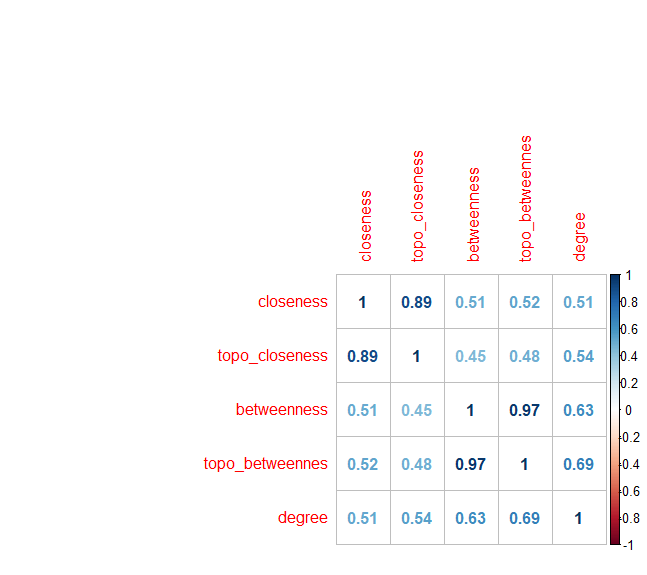
\includegraphics[width=0.8\textwidth]{Corr_tube_graph_node_stats}
\caption{Correlation between station/node metrics}
\end{figure}


\begin{center}
\csvautotabular{betfalse.csv}
\end{center}

% gotta reformat this probably asking about it on tex stack exchange

\begin{tabular}{|c|c|c|c|}\hline %
  \multicolumn{4}{|c|}{\bfseries Betweenness unconn is false}  \\ \hline
 & Node Deleted & Increase in Avg Geodesic & Components
  \csvreader[head to column names]{betfalse.csv}{} %
 {\\\index & \NodeDeleted & \IncreaseGeodesic & \Components} %
 \\\hline
 \end{tabular}
 


\begin{center}
\csvautotabular{bettrue.csv}
\end{center}

\begin{center}
\csvautotabular{eigtrue.csv}
\end{center}

\begin{center}
\csvautotabular{eigfalse.csv}
\end{center}




\subsection{Analysis}

When Kings Cross is deleted, it creates a new unconnected component out of the 11 stations on the north east end of the Picadilly line. In igraph, the two ways to handle this for the mean\_distance() function are either to exclude distances between those unconnected nodes and the rest of the network or to assume that the distance is one greater than the longest possible geodesic in the network, that is ,the number of nodes on the network. Excluding distances between unconnected nodes led to a decrease in average trip length because nodes disconnected tended to have higher than average distance to other nodes, lowering the average metric.  

Looking at the effect data it seems reasonable to say that betweenness did a better job than eigenvector centrality of prioritizing nodes to remove. Using betweenness created more isolates. It's difficult to judge which method lengthened average shortest path the most because of the options for dealing with disconnected networks. This will be discussed in the conclusion. 



\subsection{Conclusions}

To improve this work, it would be good to add data about transportation networks besides the underground. In particular information about bus routes connected nodes would be useful because it would allow for a better estimate of average shortest path when subway stations become disconnected as the shortest path could then go through a bus route instead. Similarly, it would be good to include more granular data about where a rider would have to change trains. The current network assumes there's no cost to switch trains relative to staying on the same train passing through a station. Anyone who has walked from the Picadilly line to the Northern line at Kings Cross knows that there is a big difference. 

An improvement to the data generally would be to use travel time data instead of using distance as an approximation. 

Lastly, it would be interesting to build an igraph function that can compute average shortest path using edge weights since the current function cannot. This could confirm or reject the thought that tube stations are spaced fairly regularly based on the high correlation between weighted and topological centrality measures. 

\textbf{943 words}


%%%%%%%%%%%%%%%%%%%%%%%%%%%%%%%%%%%%%%%%%%%%%%%%%%%%%%%%%%%%%%%%%%%%%%%%%%%%%
\pagebreak

\section{Part 2}

\subsection{The Models}

\subsubsection{Unconstrained}

The model is constrained to the total flows of the system but flows out of an origin and into a destination can be any value between 0 and total system flows. 

This is useful for studying the change in connectivity between regions, for instance if a new transportation link was built. In particular, it is useful for studying long term effects of a change where residence and employment are more flexible. 

\subsubsection{Production}

The direction of flows can change but the total flows from each origin will remain constant. This is useful for studying the effect of a new employment or consumption location that changes the destinations of people going to work or to spend money. In terms of the matrix, it implies that the sums of the rows of the matrix are constant. 

\subsubsection{Attraction Constrained}

The source of flows into a region can change but the total flows into a region will remain constant. That is, any reduction in flows into a destination from another region will be fully replaced by flows into the destination from another region.  This could be used to study a new housing development that pulls people into residence in a different part of an area or a natural disaster that forces residents out of an area. Employers outside the area still need workers but will not be able to draw them from the same places after a housing change or natural disaster. In terms of the matrix the sums of the columns are held constant. Additionally, it can be used to study the effect of a specific change to employment where the model can be constrained to the values that result from that change. 

\subsubsection{Doubly Constrained,}

Doubly constrained models could be used to test the short term effects of a change to transportation networks given that homes and businesses won't relocate but flexible behavior patterns like shopping could change almost immediately due to the change in accessibility or travel times between locations. In this model, the sums of both the columns and rows are held constant.

\subsection{The Parameters}

Basically, the parameters are ratios of how much a change of 1, in the natural logarithm of one of the predictor variables affects the natural log of the estimate of flow. This is seen below, 1-3 for the unconstrained and 4-6 for the doubly constrained. The equation is log-linearized and then the flow estimate is solved for. In equation 6, $A_i$ and $B_i$ are vectors of parameters that allocate parts of the regions total flows across origins and destinations and $k$ is an arbitrary intercept used for estimation. 

% basic equation
\begin{equation}
T_{ij} = k V_i ^{\mu} W_j^{\alpha} d_{ij}^{-\beta}
\end{equation}

% linear equation
\begin{equation}
ln(T_{ij}) = ln(k) + \mu (ln(V_i)) +  \alpha( ln(W_j)) - \beta (ln(d_{ij}))
\end{equation}



% solve for total flow

\begin{equation}
T_{ij} = e^ { \{ ln(k) + \mu (ln(V_i)) +  \alpha( ln(W_j)) - \beta (ln(d_{ij})) \}}
\end{equation}

% linear equation for doubly constrained model

\begin{equation}
\lambda_{ij} = A_i O_i  B_j D_j d_{ij}^{-\beta}
\end{equation}

\begin{equation}
ln(\lambda_{ij}) = ln(A_i O_i  B_j D_j) - \beta ln( d_{ij})
\end{equation}


\begin{equation}
\lambda_{ij} = A_i O_i  B_j D_j - e ^{ \beta ln( d_{ij})} + k
\end{equation}



\subsection{A Scenario}

\textit{select a scenario and explore the consequences of varying model parameters and inputs on interaction flows and the origin/destination estimates}

The scenario used for this assessment will be: ``What if teleportation  was invented and dramatically reduced travel times in connected boroughs but could only be used in London's outermost boroughs due to construction requirements?'' Thus origin and destination attributes remain constant but the travel costs change dramatically in the most peripheral boroughs: Hilingdon, Harrow, Barnet, Enfield, Waltham forest, Redbridge, Havering, Bexley, Bromley, Croydon, Sutton, Kingston, Richmond, Hounslow. 

This will be investigated using a doubly constrained model to estimate the short term effects where residences and businesses cannot relocate and a total constrained model to see the long term effects on business and residence locations as a result of the incredible new discovery. 

To approximate the effect of near instantaneous transportation between two boroughs, the lowest distance between centerpoints of two London boroughs, 2080 meters, is substituted for the real distance between each of the 9 outermost boroughs. . 

\subsection{Setup}

The two models were estimated in R. 

The parameters and goodness of fit statistics for the unconstrained model are seen in table 1. 

For the doubly constrained model, the estimated intercept was $24.63$ and distance parameter was $-1.92$. This model also produces a $32 X 32 $ matrix of origin and destination specific parameters that will not be included here. 

In both models the signs of the estimated parameters were consistent with expectations and the majority of parameters were significant at the $0.0001$ level.

\begin{center}
\begin{tabular}{lclc}
 \multicolumn{2}{l}{Parameter} 	& \multicolumn{2}{l}{Fit } \\ \hline	 
 $k$ : 		& $-12.5$ 	& RMSE :	&  $2330.9$	  	\\
 $\mu$ :	& $1.62$	& $R^2$ :	&  	$0.386$  	\\
 $\alpha$ :	& $1.55$	&  			&  	  			\\
 $\beta$ :	& $-1.5$	& 	 		&
\end{tabular}
\captionof{table}{Total constrained model results}\label{unconstrained}
\end{center} 


\subsection{Results}

\begin{sidewaystable}
\tiny
\csvautotabular{actual_flows.csv}
\end{sidewaystable}

\begin{sidewaystable}
\tiny
\csvautotabular{fit_estimate.csv}
\end{sidewaystable}

\begin{sidewaystable}
\tiny
\csvautotabular{double_estimate.csv}
\end{sidewaystable}

%\begin{table}[htbp]
%\caption{Actual Flows between boroughs}
%\begin{tabular}{|r|l|r|r|r|r|r|r|r|r|r|r|r|r|r|r|r|r|r|r|r|r|r|r|r|r|r|r|r|r|r|r|r|r|r|r|}
%\hline
%\multicolumn{1}{|l|}{} & Borough & 1 & 2 & 3 & 4 & 5 & 6 & 7 & 8 & 9 & 10 & 11 & 12 & 13 & 14 & 15 & 16 & 17 & 18 & 19 & 20 & 21 & 22 & 23 & 24 & 25 & 26 & 27 & 28 & 29 & 30 & 31 & 32 & 33 & 34 \\ \hline
%1 & Barking & 0 & 194 & 96 & 178 & 66 & 1500 & 3641 & 104 & 188 & 410 & 209 & 980 & 255 & 301 & 55 & 6415 & 97 & 91 & 1385 & 439 & 18 & 449 & 132 & 67 & 4460 & 5940 & 28 & 926 & 38 & 4069 & 1047 & 165 & 3280 & 37223 \\ \hline
%2 & Barnet & 96 & 0 & 34 & 5467 & 76 & 12080 & 7709 & 148 & 1573 & 4098 & 101 & 1576 & 1431 & 3842 & 2623 & 131 & 1023 & 611 & 5775 & 1841 & 68 & 1129 & 124 & 146 & 387 & 305 & 229 & 1792 & 44 & 2511 & 555 & 536 & 16330 & 74391 \\ \hline
%3 & Bexley & 362 & 132 & 0 & 144 & 4998 & 2470 & 6580 & 710 & 188 & 123 & 9498 & 698 & 333 & 110 & 29 & 394 & 109 & 161 & 1557 & 603 & 77 & 1808 & 2989 & 190 & 574 & 111 & 90 & 4666 & 170 & 2825 & 222 & 618 & 7692 & 51231 \\ \hline
%4 & Brent & 40 & 6124 & 28 & 0 & 66 & 8105 & 4145 & 187 & 6703 & 426 & 124 & 809 & 3709 & 730 & 5102 & 51 & 2127 & 1404 & 2535 & 3926 & 116 & 1107 & 147 & 203 & 279 & 116 & 396 & 1565 & 56 & 1655 & 210 & 669 & 16418 & 69278 \\ \hline
%5 & Bromley & 134 & 162 & 3199 & 201 & 0 & 3780 & 9855 & 6268 & 293 & 84 & 2586 & 728 & 859 & 134 & 59 & 119 & 248 & 285 & 2094 & 1241 & 227 & 3570 & 5360 & 647 & 419 & 100 & 191 & 6057 & 796 & 3385 & 196 & 1371 & 12802 & 67450 \\ \hline
%6 & Camden & 36 & 1496 & 32 & 1350 & 60 & 0 & 8795 & 147 & 643 & 295 & 140 & 1201 & 1870 & 666 & 330 & 43 & 473 & 473 & 4987 & 2267 & 89 & 1338 & 140 & 139 & 290 & 84 & 195 & 1784 & 54 & 2614 & 204 & 588 & 18829 & 51652 \\ \hline
%7 & City & 6 & 14 & 0 & 16 & 0 & 335 & 0 & 3 & 9 & 6 & 3 & 66 & 61 & 16 & 7 & 9 & 10 & 9 & 339 & 62 & 0 & 42 & 15 & 6 & 16 & 0 & 6 & 103 & 3 & 266 & 16 & 16 & 602 & 2062 \\ \hline
%8 & Croydon & 85 & 204 & 300 & 329 & 5152 & 3248 & 5925 & 0 & 405 & 120 & 523 & 599 & 1284 & 177 & 97 & 82 & 457 & 581 & 1752 & 1478 & 827 & 6844 & 1563 & 3521 & 202 & 64 & 480 & 4513 & 6744 & 2000 & 130 & 4270 & 10583 & 64539 \\ \hline
%9 & Ealing & 30 & 967 & 33 & 5263 & 91 & 4547 & 4855 & 182 & 0 & 223 & 136 & 522 & 8579 & 267 & 2601 & 48 & 13055 & 9869 & 1795 & 4111 & 364 & 1031 & 174 & 361 & 229 & 79 & 1578 & 1328 & 65 & 1420 & 127 & 944 & 13967 & 78841 \\ \hline
%10 & Enfield & 217 & 5642 & 52 & 1038 & 76 & 5588 & 5212 & 136 & 626 & 0 & 126 & 2542 & 850 & 10199 & 328 & 233 & 457 & 339 & 5317 & 1091 & 38 & 806 & 114 & 114 & 661 & 538 & 98 & 1253 & 47 & 2141 & 1710 & 314 & 9052 & 56955 \\ \hline
%11 & Greenwich & 333 & 181 & 5046 & 252 & 3196 & 3038 & 5614 & 692 & 248 & 192 & 0 & 856 & 607 & 178 & 45 & 147 & 154 & 233 & 1780 & 929 & 58 & 2292 & 5571 & 237 & 981 & 126 & 113 & 5145 & 134 & 3643 & 244 & 940 & 8847 & 52052 \\ \hline
%12 & Hackney & 222 & 687 & 56 & 514 & 90 & 7137 & 5181 & 128 & 450 & 877 & 241 & 0 & 1165 & 2335 & 92 & 124 & 203 & 283 & 7740 & 1261 & 61 & 1269 & 240 & 121 & 1069 & 402 & 149 & 2023 & 58 & 5247 & 1101 & 567 & 9983 & 51076 \\ \hline
%13 & Fulham & 25 & 259 & 19 & 812 & 56 & 4009 & 7967 & 202 & 2418 & 82 & 63 & 586 & 0 & 137 & 163 & 33 & 1090 & 2097 & 1795 & 7072 & 271 & 1153 & 122 & 466 & 123 & 33 & 854 & 1374 & 113 & 1947 & 66 & 1908 & 15305 & 52620 \\ \hline
%14 & Haringey & 144 & 3016 & 32 & 1074 & 64 & 10506 & 5523 & 213 & 668 & 4249 & 154 & 3130 & 1486 & 0 & 268 & 99 & 330 & 450 & 7948 & 1889 & 67 & 1236 & 178 & 136 & 520 & 278 & 180 & 1857 & 48 & 2350 & 1004 & 507 & 13479 & 63083 \\ \hline
%15 & Harrow & 55 & 5008 & 26 & 9473 & 47 & 3675 & 3162 & 103 & 4542 & 325 & 62 & 430 & 1487 & 331 & 0 & 29 & 6169 & 1141 & 1395 & 1160 & 107 & 501 & 71 & 119 & 99 & 44 & 246 & 854 & 34 & 1013 & 95 & 300 & 7882 & 49985 \\ \hline
%16 & Havering & 7278 & 194 & 325 & 156 & 157 & 2001 & 8348 & 131 & 165 & 546 & 260 & 1302 & 260 & 335 & 69 & 0 & 116 & 83 & 1932 & 358 & 33 & 552 & 137 & 85 & 3410 & 4844 & 45 & 1389 & 50 & 5030 & 1173 & 158 & 4699 & 45621 \\ \hline
%17 & Hillingdon & 31 & 692 & 18 & 2672 & 55 & 1757 & 1661 & 116 & 8185 & 153 & 49 & 205 & 1799 & 110 & 4688 & 21 & 0 & 5293 & 664 & 925 & 150 & 401 & 79 & 167 & 83 & 35 & 548 & 511 & 58 & 565 & 53 & 248 & 5062 & 37054 \\ \hline
%18 & Hounslow & 19 & 253 & 27 & 807 & 69 & 1753 & 2342 & 215 & 5488 & 92 & 106 & 250 & 3587 & 87 & 396 & 28 & 12803 & 0 & 752 & 1800 & 1006 & 692 & 128 & 303 & 100 & 31 & 7025 & 657 & 101 & 753 & 41 & 765 & 5927 & 48403 \\ \hline
%19 & Islington & 110 & 1001 & 46 & 538 & 46 & 10188 & 7931 & 157 & 479 & 619 & 138 & 2758 & 1473 & 1869 & 111 & 55 & 265 & 334 & 0 & 1672 & 50 & 1191 & 152 & 131 & 348 & 117 & 118 & 1883 & 56 & 2837 & 393 & 490 & 12835 & 50391 \\ \hline
%20 & K and C & 22 & 232 & 20 & 548 & 64 & 3554 & 10098 & 165 & 861 & 48 & 54 & 445 & 3679 & 123 & 106 & 18 & 576 & 788 & 1816 & 0 & 112 & 1029 & 78 & 208 & 68 & 30 & 300 & 1168 & 67 & 2957 & 68 & 1085 & 15947 & 46334 \\ \hline
%21 & Kingston & 9 & 104 & 35 & 184 & 72 & 1547 & 2875 & 638 & 469 & 42 & 58 & 176 & 1327 & 32 & 68 & 24 & 1070 & 1484 & 710 & 847 & 0 & 1028 & 70 & 3041 & 71 & 31 & 3788 & 1038 & 1190 & 825 & 20 & 2395 & 5419 & 30687 \\ \hline
%22 & Lambeth & 64 & 406 & 136 & 477 & 826 & 8090 & 9697 & 3143 & 667 & 150 & 595 & 1469 & 3376 & 373 & 89 & 49 & 466 & 898 & 4149 & 4368 & 527 & 0 & 1344 & 1830 & 380 & 123 & 855 & 8267 & 803 & 3414 & 185 & 8028 & 24349 & 89593 \\ \hline
%23 & Lewisham & 164 & 271 & 1170 & 332 & 6677 & 4963 & 7251 & 2457 & 457 & 133 & 4555 & 1231 & 1114 & 277 & 83 & 93 & 238 & 365 & 2669 & 1791 & 181 & 5685 & 0 & 583 & 657 & 141 & 259 & 11118 & 406 & 3949 & 236 & 1901 & 13727 & 75134 \\ \hline
%24 & Merton & 34 & 181 & 56 & 251 & 316 & 2952 & 6051 & 3193 & 554 & 49 & 176 & 454 & 2310 & 143 & 68 & 20 & 532 & 848 & 1411 & 2223 & 3516 & 3383 & 250 & 0 & 157 & 31 & 1334 & 2282 & 3743 & 1704 & 81 & 8410 & 10148 & 56861 \\ \hline
%25 & Newham & 2702 & 401 & 147 & 513 & 207 & 3855 & 5009 & 190 & 431 & 584 & 735 & 2397 & 741 & 675 & 57 & 934 & 207 & 283 & 2709 & 1497 & 86 & 1154 & 386 & 139 & 0 & 2969 & 126 & 2089 & 56 & 9120 & 2161 & 534 & 8565 & 51659 \\ \hline
%26 & Redbridge & 4664 & 567 & 141 & 386 & 132 & 3790 & 8205 & 173 & 343 & 1187 & 330 & 2338 & 581 & 906 & 110 & 3004 & 212 & 231 & 3104 & 746 & 46 & 853 & 188 & 100 & 6031 & 0 & 88 & 1760 & 48 & 6916 & 5441 & 262 & 8122 & 61005 \\ \hline
%27 & Richmond & 15 & 173 & 12 & 342 & 64 & 2504 & 4831 & 323 & 1469 & 41 & 64 & 276 & 3181 & 53 & 167 & 20 & 3365 & 6873 & 1002 & 1745 & 3549 & 1216 & 84 & 840 & 65 & 12 & 0 & 1213 & 260 & 1197 & 46 & 1991 & 8336 & 45329 \\ \hline
%28 & Southwark & 108 & 319 & 281 & 428 & 933 & 6003 & 9041 & 1213 & 536 & 135 & 1138 & 1401 & 1682 & 271 & 123 & 74 & 312 & 466 & 3203 & 2552 & 273 & 8500 & 3163 & 566 & 580 & 161 & 313 & 0 & 261 & 4243 & 251 & 2545 & 16500 & 67575 \\ \hline
%29 & Sutton & 33 & 81 & 68 & 138 & 514 & 1450 & 2560 & 7602 & 309 & 45 & 101 & 230 & 851 & 51 & 50 & 23 & 385 & 541 & 681 & 882 & 3122 & 1827 & 270 & 6725 & 95 & 26 & 750 & 1404 & 0 & 872 & 41 & 3217 & 4691 & 39635 \\ \hline
%30 & Tower Hamlets & 370 & 257 & 140 & 192 & 192 & 4080 & 10104 & 183 & 291 & 224 & 275 & 2668 & 935 & 326 & 56 & 304 & 146 & 245 & 3235 & 1249 & 58 & 1090 & 316 & 124 & 1845 & 407 & 151 & 2182 & 55 & 0 & 562 & 405 & 9304 & 41971 \\ \hline
%31 & Waltham Forest & 846 & 715 & 79 & 491 & 149 & 5554 & 6337 & 253 & 440 & 2661 & 337 & 3957 & 832 & 2467 & 112 & 594 & 206 & 271 & 4310 & 1378 & 50 & 1059 & 228 & 122 & 3257 & 3736 & 101 & 1719 & 41 & 4789 & 0 & 409 & 10314 & 57814 \\ \hline
%32 & Wandsworth & 34 & 297 & 69 & 422 & 324 & 7140 & 13935 & 1496 & 970 & 116 & 256 & 1044 & 6232 & 225 & 129 & 31 & 853 & 1690 & 3404 & 6208 & 1806 & 5951 & 403 & 4329 & 208 & 59 & 2338 & 4092 & 992 & 4024 & 135 & 0 & 24409 & 93621 \\ \hline
%33 & Westminster & 25 & 514 & 17 & 1229 & 99 & 6786 & 9521 & 216 & 925 & 121 & 93 & 745 & 2369 & 228 & 142 & 26 & 597 & 572 & 2442 & 4767 & 90 & 1381 & 148 & 178 & 170 & 60 & 258 & 1663 & 61 & 2851 & 121 & 873 & 0 & 39288 \\ \hline
%34 & (all) & 18313 & 30744 & 11740 & 36217 & 24934 & 147985 & 209961 & 31087 & 41993 & 18456 & 23286 & 38069 & 60305 & 27974 & 18423 & 13275 & 48351 & 39292 & 86387 & 64378 & 17043 & 61567 & 24364 & 25944 & 27834 & 21033 & 23230 & 79675 & 16652 & 93132 & 17935 & 47429 & 353405 & 1800413 \\ \hline
%\end{tabular}
%\label{Actual Flows}
%\end{table}








%%%%%%%%%%%%%%%%%%%%%%%%%%%%%%%%%%%%%%%%%%%%%%%%%%%%%%%%%%%%%%%%%%%%%%%%%%%%%

\section{Part 3}

\subsection{Overview}

While CA models are often viewed as separate from ABM, a more modern view of these methods considers them to be cousins or related in the sense that CA are a subset of ABM. 

Expanding a CA model usually results in the creation of an ABM.  Cellular automata models are defined by a set of homogeneous cells that interact only with each other according to a defined set of input/output functions, e.g., if a cell with value 1 is surrounded by other cells f value 1 it's value becomes 0. The models can be extended to "n" states but all cells should be capable of reaching all n states to maintain the homogeneity of the cells. This can be contrasted with ABM where cells can have infinite heterogeneity and future states can be functions of the "environment" other cells or agents" and the cells own state. 

The simplicity of CA models make them very useful for studying mathematical processes whereas Agent Based Modeling flexibility make them useful for modeling more complex "real world" phenomena and make them more accessible to non-technical audiences. Often the value of ABM comes from the ability to conduct parameter sweeps, to study combination rules that apply to multiple conceptual processes with different parameter values. The value of cellular automata models tends to be focused on the effect of initialization states on the long term outcomes and equillibria of the model e.g. for the same model, outcomes are a function of the rule set and initialization values, where as agent based models tend to be calculated for a large number of initialization values in order to study the effect of model dynamics independent of initialization values that may not accurately reflect the real world. 

\subsection{Scenarios}

This work will investigate three possible infection scenarios. The first is a baseline scenario used to explore a moderately recoverable disease to which immunity is low, for instance the seasonal flu without a vaccination program. The second scenario looks at the same disease with a vaccination program. The third looks at a disease like the common cold which is more recoverable but where immunity is close to non-existent. 

All three scenarios will use a population of 1000 and infect 100 people initially. 

\subsubsection{Scenario 1}
%%%%%%%%%%%%%%%%%%%%%%
% describe 

The first scenario, looking at a flu type disease with no vaccine available uses 50\% chance of immunity, based on the idea that it's fairly common for someone with the flu to interaction with someone else without infecting them and a 10\% chance of recovery based on the guess that flu symptoms last between 3 and 9 days for the majority of the population.

% time required to reach steady state

Looking at Figure 2, which plots the percentage of turtles infected over 150 steps of the model for 20 trials, a steady state becomes fairly clear. While this is not a perfect equilibrium, compared to the rapid increase in the first 20 ticks, the model becomes fairly stationary.  This, future runs of this model can be limited to 40 ticks with reasonably confidence that the model will have found an equilibrium. 

\begin{figure}
\centering
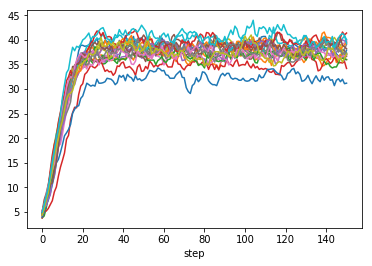
\includegraphics[width=0.8\textwidth]{scen_1_steady_state}
\caption{\% of Population Infected Over Time \\ Scenario 1}
\end{figure}


% minimum runs for statistically meaningful results

The average steady state percentage of turtles infected at 50 ticks was 38.79. The sample standard deviation was 1.799, which indicates a margin of error at 95\% confidence of $\pm 0.842$ using a t-value of 2.093. This implies that to get a margin of confidence of 0.5, 56.7 trial runs would be required. When 56 trials were run, the result was $37.93 \pm 0.493$, so the estimate for $n$ was pretty accurate. 

The total infection time per non-immune turtle per tick was also recorded. The 20 trial mean at tick 40 was $0.6343 \pm 0.00669$. This has the value of adjusting for turtle immunity and runtime in order to compare results across scenarios later on. 

% conclusions. 

Thus the model indicates that for these parameters, a fairly high number of turtles will contract the infection and the infection will be passed around continually rather than dying out at some point in the future. Considering the margin of errors for the results, if the model accurately reflects a real world scenario, we can have a good idea of how that scenario would play out. 

\subsubsection{Scenario 2}
%%%%%%%%%%%%%%%%%%%%
% describe

Scenario 2 looks at the flu in a society with high but imperfect immunization rates. In the US this is seen in cases where infants and the elderly cannot receive the vaccine and some people elect not to receive it or forget. This is accomplished by using the same recovery rate, 10\% but increasing immunity probability to 80\%. 


% time required to reach steady state

In Figure 3 the distribution over time of the percentage of turtles infected in the scenario is illustrated. It can be seen that a steady state is more difficult to identify. One consideration is that the average percentage is lower than in scenario 1 because 80\% of the population is immune. A second is that the lower mean scales the y-axis of the chart down from 0-14 instead of 0-45 in scenario 1. Thus while the standard deviation looks higher it is essentially the same, 1.869 in scenario 1 and 1.853 in scenario 2. 

Because a steady state is less certain looking at the chart a t-test can be used to confirm that the mean of the set of trials is not changing between steps. At step 50 the mean percent infected was 5.92 with st. deviation 1.799. At step 100 these were 6.90 and 1.99. At step 250 7.935 and 1.696. At step 400 8.075 and 1.502. At step 500 7.956 and 2.113. 

The p-value for a t-test with the null hypothesis that the means at steps 50 and 100 are different was 0.116. Indicating a 12\% chance that they are different and that a steady state has not been reached with 95\% confidence. The same test for the means at tick 250 and tick 500 had a p-value of 0.97. The test for steps 400 and 500 had a p-value of 0.84. Thus it is difficult to say with confidence that a steady state exists for this model as the effort to reject the null hypothesis that the means are different begins to resemble simply getting lucky enough to choose ticks with means that are very similar to each other by coincidence. 

Sicktime per turtle per tick at 100 ticks was $ 0.1047 \pm 0.01397$. A lower average sicktime compared to scenario 1 with not as tight confidence interval. 

\begin{figure}
\centering
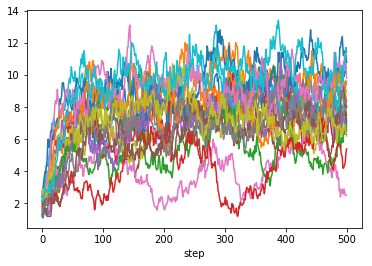
\includegraphics[width=0.8\textwidth]{20-runs-scenario-2-steady-state}
\caption{\% of Population Infected Over Time \\ Scenario 2}
\end{figure}


% minimum runs for statistically meaningful results

at tick 250, the mean percentage of turtles infected was $7.94 \pm 0.794$ again demonstrating that the variability in results for this scenario is very similar to those of scenario 1 but that in light of the results of a t-test for a steady state, the true margin of error is likely to be higher since the process may not be stationary at tick 250, that is to say, the true mean may change across ticks.  Finally, smaller sets of trials exhibited similar results to those calculated in scenario 1 showing that the change in parameters affected the value of the results but not their variability. 

\subsubsection{Scenario 3}

% describe

This scenario will investigate how the common cold compares to the flu by using a higher rate of recovery 25\% and lower rate of immunity 5\% since there is no vaccine for the common cold and many members of society continue their daily routines after contracting it exposing relatively more people than the flu, which most people suffer at home. 

% time required to reach steady state

Figure 4 illustrates the percentage of turtles infected over time. Here a steady state seems more obvious. At 50 ticks the mean was 66.19 and st. deviation was 1.597. At 100 ticks this was 65.84 and 1.648. The 0.04994 p-value for a two tailed t-test for difference in means indicates only a 5\% probability of the null hypothesis that the means are different, just on the border of an acceptable level of confidence but basically acceptable.

\begin{figure}
\centering
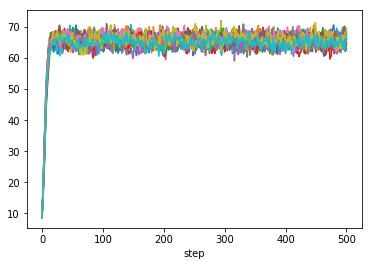
\includegraphics[width=0.8\textwidth]{20-runs-scenario-3-steady-state}
\caption{\% of Population Infected Over Time \\ Scenario 3}
\end{figure}

% minimum runs for statistically meaningful results

At 50 ticks the mean percentage of turtles infected was $66.08 \pm 0.902$ . Thus the low variability of outcomes for different outcome values as a result of different parameter values continues. 

Results for sick time per turtle per tick at tick 50 were $0.311 \pm 0.0013$. Less than the no vaccine flu scenario. which was less recoverable but more than the vaccinated scenario. 


\subsection{Conclusion}

Comparing the three scenarios, The unvaccinated flu, scenario 1, (moderate immunity (50\%) and moderate recovery rates (10\%)) resulted in a 38\% average infection rate while the vaccinated flu (80\% immunity and 10\% recovery) resulted in 7.93\% of turtles infected on average. The common cold, (5\% immunity, 25\% chance of recovery) gave 66\% of turtles infected. At tick 50, non-immune turtles in scenario 1 had spent 63\% of ticks infected on average while this number was  10\% in scenario 2 and 31\% in scenario 3, demonstrating the value of population immunity to non-immune members. 

Scenario 1 turtles that were not immune had spent $23.6 \pm 0.12$ ticks sick on average while this was $7.54 \pm 0.45$ in scenario 2 and $24.14 \pm 0.05$ in scenario 3. 

Thus it is clear that higher rates of vaccination in scenario 2 lead to lower amounts of sicktime for turtles without the vaccine. At a high level it can then be said that this model replicates the empirical idea of ``herd immunity'' where general immunity of a group protects non-immune members of the group. 

To continue investigating this, the model could be explored to find whether there is a constant increase in sick time per non-immune turtle or whether as population immunity decreases sick time accelerates. It would also be useful to add in a parameter for the contagiousness of the infection, the radius within which turtles affect each other. Lastly, adding in death or post-infection immunity would be an interesting extension. 


\textbf{1618 words}


\nocite{*}


\printbibliography


\end{document}
